% ============================================= %

\documentclass[12pt,a4paper]{report}
\usepackage{graphicx}
\usepackage{amsmath}
\usepackage{fancyhdr}
\usepackage{cite}
\usepackage{framed}
\usepackage{a4wide}
\usepackage{float}
\usepackage{epsfig}
\usepackage{longtable}
\usepackage{enumerate}
\usepackage{afterpage}
\usepackage{multirow}
\usepackage{ragged2e}
\usepackage{gensymb}
\usepackage{amsfonts} 
\usepackage[left=2.54cm,top=2.54cm,right=2.54cm,bottom=2.54cm]{geometry}
\usepackage{setspace}           
\usepackage{float}
\usepackage{txfonts}
\usepackage{lipsum}
\usepackage{indentfirst}
\newcommand{\Usefont}[1]{\fontfamily{#1}\selectfont}

\usepackage{lscape} % for landscape tables
\renewcommand{\baselinestretch}{1} 

\usepackage{blindtext}
\usepackage{xpatch}
\usepackage{url}
\usepackage{leqno}
\usepackage{subcaption}
\linespread{1.2}
\usepackage[intoc, english]{nomencl}
\hyphenpenalty=5000
\tolerance=1000
\usepackage[nottoc]{tocbibind}
\bibliographystyle{IEEEtran}
\renewcommand{\bibname}{References}

\usepackage{titlesec}

% format for unnumbered chapter titles
\titleformat{name=\chapter,numberless}[block]
{\centering\normalfont\LARGE\bfseries}{}{0pt}{\Huge}
\titlespacing*{name=\chapter,numberless}     {0pt}{-20pt}{20pt}

% format for numbered chapter titles
\titleformat{\chapter}[display]
{\filcenter\normalfont\Huge\bfseries}
{\vspace*{\fill}{\chaptertitlename} \thechapter}
{0pt}{\Huge}[\vspace*{\fill}\newpage]
\titlespacing*{\chapter}{0pt}{-50pt}{0pt}

% \usepackage{blindtext}
% \usepackage{showframe}

\usepackage{listings}
\lstset{
  columns=flexible,
  basicstyle=\small\ttfamily,
  mathescape=true,
  escapeinside=||
}

\usepackage{tikz}
\usepackage{eso-pic}
\usetikzlibrary{calc}
\usetikzlibrary{decorations.pathmorphing}
% \AddToShipoutPictureBG{\ifnum\value{page}<2 % <- change this if you want more
% % or less pages to have a frame
% \begin{tikzpicture}[overlay,remember picture]
% \draw [line width=3pt]
%       ($ (current page.north west) + (1.5cm,-1.5cm) $)
%     rectangle
%     ($ (current page.south east) + (-1.5cm,1.5cm) $);
% \draw [line width=1pt]
%     ($ (current page.north west) + (1.65cm,-1.65cm) $)
%     rectangle
%     ($ (current page.south east) + (-1.65cm,1.65cm) $); 
% \end{tikzpicture}%
% \fi}


% ================== Figures ================== %

 
% Save all figures in the folder figures and
% include them in your report using the
% command \includegraphics{figure-name}

\graphicspath{{figures/}}

% figure files can be in jpeg,jpg, png or 
% pdf formats


\begin{document}
	
% ============== Global Variables ============= %

% The entries in this section are to be filled 
% in by the student with appropriate values

% These values are used throughout the report 

% please fill in the appropriate values in the 
% brackets {}

% Project title
\gdef \title{Technical Project Report Template using Latex} 

% Department
\gdef \dept{Information Technology} 
% Degree
\gdef \degree{Bachelor of Engineering} 
% Branch
\gdef \branch{Information Technology} 

% Name of the College
\gdef \college{Bharati Vidyapeeth College of Engineering} 
% Location of the College
\gdef \collegeplace{Navi Mumbai} 

% Project group member 1
\gdef \studentA{Bhoir Ankit Bharat} 
% Project group member 1 roll number
\gdef \studentAroll{4407} 

% Project group member 2
\gdef \studentB{Ankolekar Vaibhav Pandurang} 
% Project group member 2 roll number
\gdef \studentBroll{4401} 

% Project group member 3
\gdef \studentC{Chouhan Aman Ravi} 
% Project group member 3 roll number
\gdef \studentCroll{4414} 

% Project group member 4
\gdef \studentD{Badge Aman Ramesh} 
% Project batch member 4 roll number
\gdef \studentDroll{4404} 

% Project guide
\gdef \guide{Prof. Hanamant B. Sale}
% Project guide designation
\gdef \guidedes{Subject Co-ordinator}

% Project external organisation guide
\gdef \guideext{Prof. Project External Guide} 
% project external guide designation
\gdef \guideextdes{External}

% Head of Department
\gdef \hod{Dr. Shankar M. Patil} 
% HOD designation
\gdef \hoddes{Head of Department} 

% Academic year
\gdef \acadyear{2022 - 23} 
% Month of Report submission
\gdef \month{October 2022} 
% Date of signing the declaration
\gdef \date{04-10-2022} 

% ================ Cover Page ================= %

% The font pages. The source tex files are there 
% in the folder


% =============== coverpage.tex =============== %
  

\newenvironment{coverpage}
\thispagestyle{empty}
\begin{titlepage}
	\begin{center}
        
        \begin{tikzpicture}[overlay,remember picture]
        \draw [line width=3pt]
               ($ (current page.north west) + (1.3cm,-1.3cm) $)
            rectangle
            ($ (current page.south east) + (-1.3cm,1.3cm) $);
        \draw [line width=1pt]
            ($ (current page.north west) + (1.45cm,-1.45cm) $)
            rectangle
            ($ (current page.south east) + (-1.45cm,1.45cm) $); 
        \end{tikzpicture}
        
		{\Usefont{phv} \Large \bf{\title} \par}
		\vspace*{40pt}
		\large \em \Usefont{pzc}{ 
			A Project Report \par
			Submitted to the \college \\
			in partial fulfillment of requirements for the award of degree}\\ [.15\baselineskip]
		\vspace*{30pt}
		\Usefont{ppl} {\bfseries  \degree}\\
		in\\
		{\Usefont{ppl} {\bfseries \branch}}\\
		\vspace*{20pt}
		by\\
		\vspace*{30pt}
		\bf {\studentA} (\studentAroll)\\
		\bf {\studentB} (\studentBroll)\\
		\bf {\studentC} (\studentCroll)\\
		\bf {\studentD} (\studentDroll)\\
		\vspace*{40pt}
		\centering
		\begin{figure}[h!]
			\centerline{
\includegraphics[scale=0.5]{bvcoe_logo}}
		\end{figure}
		
		\vspace{\stretch{0.5}}
		\footnotesize{\bf DEPARTMENT OF \MakeUppercase{\dept}} \par
		\bf{\MakeUppercase{\college}} \par
		\bf{\MakeUppercase{\collegeplace}} \par
		\bf{\month}
	\end{center}		
\end{titlepage}	
 

% Unless essential Do not edit this tex file

% ================ Certificate ================ %

% ==================================certificate1.tex================================
% To print name of only the seminar coordinator 1 in the certificate page

\newpage

\begin{tikzpicture}[overlay,remember picture]
\draw [line width=3pt]
       ($ (current page.north west) + (1.3cm,-1.3cm) $)
    rectangle
    ($ (current page.south east) + (-1.3cm,1.3cm) $);
\draw [line width=1pt]
    ($ (current page.north west) + (1.45cm,-1.45cm) $)
    rectangle
    ($ (current page.south east) + (-1.45cm,1.45cm) $); 
\end{tikzpicture}
        
\begin{center}	
    \textbf{DEPARTMENT OF \MakeUppercase{\dept}} \\	
	\textbf{\MakeUppercase{\college}} \\
	\textbf{\MakeUppercase{\collegeplace}} \\
	\textbf{\acadyear} 
\end{center}

\vspace{20pt}

\begin{center}
	
\includegraphics[scale=0.38]{bvcoe_logo}	
\end{center}

\vspace{20pt}

\begin{center}
	\textbf{CERTIFICATE}
\end{center}

This is to certify that the report entitled \textbf{\title} submitted by \textbf{\studentA}\hspace*{2pt}(\studentAroll),\hspace*{2pt}\textbf{\studentB}\hspace*{2pt}(\studentBroll),\hspace*{2pt}\textbf{\studentC}\hspace*{2pt}(\studentCroll) and \textbf{\studentD}\hspace*{2pt}(\studentDroll) to the Bharati Vidyapeeth College of Engineering in fulfillment of the B.E.\ degree in \branch \hspace*{2pt} is a bonafide record of the project work carried out by him under our guidance and supervision. This report in any form has not been submitted to any other University or Institute for any purpose.


\begin{singlespace}
	\vspace*{3cm}
	\begin{table}[h!]
		\centering
		\begin{tabular}{c p{3cm} c} 
			\textbf{\guide} & &  \textbf{\hod}\\
			(\guidedes)     & & (\hoddes)
		\end{tabular}
		
	\end{table}
	
	\vspace*{3cm}
	
	\begin{center}
		(\guideextdes)\\
	\end{center}
\end{singlespace}

\thispagestyle{empty}



 

% ================ Declaration ================ %

% Unless essential Do not edit this tex file

% ==================================declaration.tex================================ %

\newpage
\newenvironment{declaration}
\thispagestyle{empty}


\begin{tikzpicture}[overlay,remember picture]
    \draw [line width=3pt]
           ($ (current page.north west) + (1.3cm,-1.3cm) $)
        rectangle
        ($ (current page.south east) + (-1.3cm,1.3cm) $);
    \draw [line width=1pt]
        ($ (current page.north west) + (1.45cm,-1.45cm) $)
        rectangle
        ($ (current page.south east) + (-1.45cm,1.45cm) $); 
\end{tikzpicture}

\begin{center}
\Large
\textbf{DECLARATION}\\
\end{center}

\vspace*{20pt}

We hereby declare that the project report {\bf{\title}}, submitted for partial fulfillment of the requirements for the award of degree of \degree \ of the \college, \collegeplace \ is a bonafide work done by us under supervision of \guide \hspace*{2pt} \\

This submission represents our ideas in our own words and where ideas or words of others have been included, we have adequately and accurately cited and referenced the original sources. \\

We also declare that we have adhered to ethics of academic honesty and integrity and have not misrepresented or fabricated any data or idea or fact or source in my submission. We understand that any violation of the above will be a cause for disciplinary action by the institute and/or the University and can also evoke penal action from the sources which have thus not been properly cited or from whom proper permission has not been obtained. This report has not been previously formed the basis for the award of any degree, diploma or similar title of any other University.

\noindent \begin{minipage}{0.45\linewidth}
\begin{flushleft}
\vspace{7.5cm}

\collegeplace \\
\date

\end{flushleft} 
\end{minipage}
\hfill
\begin{minipage}{0.45\linewidth}
\begin{flushright}                                      
\vspace{6cm}

\textbf{\studentA}\\
\textbf{\studentB}\\
\textbf{\studentC}\\
\textbf{\studentD}\\


\end{flushright} 
\end{minipage}
\thispagestyle{empty}
 

\pagenumbering{roman} 

% ================== Abstract ================= %

% Please type in the abstract in abstract.tex file

% ===================== abstract.tex ===================== %
\chapter*{Abstract}
\addcontentsline{toc}{chapter}{Abstract}%

This document contains essential templates required to write technical reports using \LaTeX. This template may be used for the preparation of B.Tech project reports of Bharati Vidyapeeth College of Engineering, Navi Mumbai. Also minimum working examples to create equations, include figure, include table, table of contents symbols list and bibliographic citation in a \LaTeX \ document are provided. \\

Students taking the undergraduate degrees in Engineering at the Bharati Vidyapeeth College of Engineering are required to undertake several a projects and to write them up as reports. This document provides some advice on using \LaTeX \ to typeset these reports. It is also an example of how to go about making a \LaTeX \ document: you should read the source as well as the typeset document in order to see how it was all done. This document originally conformed to the regulations laid down for the project report: it had the correct font size, margins etc. So you could use it as a template for your project report by removing all of our content and inserting your own. You should check with the current course organiser for projects whether this is still true. \\

\thispagestyle{plain}
%=======================================================================

 

% ============== Acknowledgement ============== %

% Unless essential Do not edit this tex file


% ============ acknowledgement.tex ============ %
  
\chapter*{Acknowledgement}
\addcontentsline{toc}{chapter}{Acknowledgement}%

It gives us a great sense of pleasure to present the report of the B.E Project undertaken during \degree \ Final Year. We owe special debt of gratitude to \guide, \guidedes, \dept, \college, \collegeplace \ for his constant support and  guidance throughout the course of our work. His sincerity, thoroughness and perseverance have been a constant source of inspiration for us. It is only his cognizant efforts that our endeavors have seen light of the day. \\

We also take the opportunity to acknowledge the contribution of \hod, \hoddes, \dept, \college, \collegeplace \ for his full support and assistance during the development of the project. \\

We also do not like to miss the opportunity to acknowledge the contribution of all faculty members of the department for their kind assistance and cooperation during the development of our project. Last but not the least, we acknowledge our friends for their contribution in the completion of the project. \\

\vspace*{120pt}
\begin{flushright}
	\textbf{\studentA}\\
	\textbf{\studentB}\\
	\textbf{\studentC}\\
	\textbf{\studentD}\\
\end{flushright}
\thispagestyle{plain}
  

\thispagestyle{empty}
\newpage
    
% ============= Table of Contents ============= %

  
\tableofcontents
\listoffigures
\listoftables

% List of Symbols (Optional) 
% comment if not required.
% %==================================symbols.tex================================
% List of Symbols
\chapter*{List of Symbols}
\addcontentsline{toc}{chapter}{List of Symbols}%
%\makeatletter
%
%\makeatother
%%\newcommand{\abbrlabel}[1]{\makebox[3cm][l]{\textbf{#1}\ \tocfill}}

\newenvironment{symbols}

		
\begin{itemize} \setlength{\itemsep}{0pt}
	\item [$\Omega$] \text{Unit of Resistance}
	\item [$\varepsilon^{'}$]  Real part of dielectric constant
	\item [$\mbox{c}$]	Speed of light
	\item [$\lambda$] Wavelength
	\item [$\delta$] Delta
\end{itemize}
		
%\begin{symbols}
%	\item \symbol{$\Omega$} \text{Unit of Resistance}
	
%	\item \symbol{[$\mu$]} 	\text{Magnetic permeability}
%	\item[$\mu_0$]	Magnetic permeability of free space
%	\item[$\varepsilon$] Relative complex dielectric constant
%	\item[$\varepsilon^{'}$]  Real part of dielectric constant 
%	\item[$\varepsilon^{''}$] Imaginary part of dielectric constant 
%	\item[$\varepsilon_{s}$] Snow surface dielectric constant
%	\item[$\mbox{c}$]	Speed of light
%	\item[$\lambda$]	Wavelength
%	\item[$\tau$] Pulse length of SAR signal
%	\item[$\beta$]  Bandwidth of the SAR signal
%	\item[$\theta$ ] 	Orientation angle 
%	\item[$\theta_{i}$] 	Incidence or local incidence angle
%	\item[$\theta_{r}$]  Local refractive angle 
%	\item[$\delta A$]	Azimuth resolution of the SAR data
%	\item[$L$]    SAR antenna length
%	\item[$\mathbf{E}(\mathbf{r},t)$] Electric field vector
%	\item[$\mathbf{E_{pq}^s}$]	Scattered field vector
%	\item[$\rho(\mathbf{r}, t)$] Volume density of free charges
%	\item[$\mathbf{g}_\mathbf{E}$] Stokes vector


 %
% symbol should be added in the file symbol.tex

% ============= Body of the report ============ %

% Arabic numbering is used in the body of the 
% report
\cleardoublepage
\setcounter{page}{1}
\pagenumbering{arabic}

% ================= Chapter 1 ================= %

% add Introduction of your project in 
% introduction.tex file

\chapter{Introduction}

The generally used documents such as project reports, notices, internal notes etc. in any technical institute are expected to be submitted in a standard specified format. The commonly used editing tools for this purpose are Microsoft Word, notepad, wordpad, etc. Taking into consideration various formatting constraints namely alignment, font styles, paragraphs, sections, subsections, etc. becomes a bit tedious using MS Word or other tools. Also maintaining the subscripts and superscripts to obtain the various mathematical equations becomes difficult and time consuming. \\

To overcome this drawback we have \LaTeX \, a documentation preparation system that enables the document writer to concentrate on the contents of their text, without bothering too much about the formatting of it. 

\section{\LaTeX \ : what is it?}

\LaTeX \ is a document preparation system for high-quality typesetting. It is most often used for medium-to-large technical or scientific documents but it can be used for almost any form of publishing. \\

\LaTeX \ is not a word processor. \LaTeX \ is based on the idea that authors should be able to focus on the content of what they are writing without being distracted by its visual presentation. In preparing a \LaTeX \ document, the author specifies the logical structure and lets the \LaTeX \ system worry about the presentation of these structures. It therefore encourages the separation of layout from content while still allowing manual typesetting adjustments where needed. \\

\LaTeX \ is based on Donald E. Knuth’s TEX typesetting language or certain extensions. \LaTeX \ was first developed in 1985 by Leslie Lamport. 

\section{What are the advantages and disadvantages?}

You might want to consider using \LaTeX \ for your project write-up and your other reports for the following reasons:

\begin{itemize}
    \item The typeset text looks nicer than word-processor output.
    \item The table of contents, cross-references and bibliography can be generated automatically. 
    \item Many journals provide \LaTeX \ styles and templates, so that when you come to write scientific papers you can do so in \LaTeX \ without thinking about the typesetting at all. \LaTeX \ is threfore a useful skill to have learned for any career in the hard sciences.
    \item \LaTeX \ is available for FREE, for all popular operating systems (and most of the unpopular ones).
    \item The \LaTeX \ way of typesetting equations occurs in other contexts, e.g. markdown cells in jupyter notebooks and any text items in matplotlib plots.
    \item You like programming. You hate word processors and find them frustrating.
\end{itemize}
Reasons that you might not want to choose \LaTeX \ include:
\begin{itemize}
    \item \LaTeX \ is not WYSIWYG. You type your document into an ordinary text editor and typeset it in a separate step. Arguably, this helps one to separate layout (the computer’s job) from content (your job). 
    \item While it is easy to get \LaTeX \ to typeset your document in its default style, it can be tiresome or obscure to get it to do anything different.
    \item The learning curve can be a little steep at first.
    \item You like word processors. You are good at getting them to do your bidding. You want to make use of this expertise.
\end{itemize}

\section{Why \LaTeX \ ?}

What you see is what you get (WYSIWYG) programs make it easy to put text wherever you want in whatever size and style of type you want, i.e., WYSIWYG programs offer visual design. The visual design is fine for short, simple documents like letters and memos. The visual design is not good for more complex documents such as scientific papers. For this purpose, we use \LaTeX \ that offers logical design. \\

\LaTeX \ is intended to provide a high-level language that accesses the power of TEX. \LaTeX \ comprises a collection of TEX macros and a program to process \LaTeX \ documents. Because the TEX formatting commands are very low-level, it is usually much simpler for end-users to use \LaTeX \ . As \LaTeX \ is distributed under the terms of the \LaTeX \ Project Public License (LPPL), \LaTeX \ is free software.

\section{Required Parts of \LaTeX \ input file}

A few commands must appear in every \LaTeX \ input file in a certain order. They are: \\
\\
\verb|\documentclass{classname}|\\
\verb|\begin{document}|\\
\verb|\end{document}|\\

\par The documentstyle has a required argument stylename to select an overall type-setting style for the document; the one normally used is article (there are also book, report, letter, and memo). It also has an optional argument to select 11pt or 12pt normal type size (10pt is the default size). The actual text of user document and associated commands go between the begin and end commands.

\section{Customizing \LaTeX}

There are situations where LATEXdoes not provide a command or environment that matches user needs, or the output produced by some existing command may not meet user requirements. To add your own commands, use \\
\\
\verb|\newcommand{name}[num]{definition}| \\

\par The command requires two arguments: the name of the command you want to create, and the definition of the command. The num argument in square brackets is optional. 

\section{Creation of style file}

Typically, a style sheet is specified at the beginning of document. This style sheet applies to the entire document. To create your own style file, at the very beginning of the text document just write,\\ 
\\
\verb|\ProvidesPackage{mypack}|\\

\par where mypack is the name of package. Write whatever you want in it using all the LATEXcommands you know. The style file should have the same name as that of the package name. Save this style file with extension .sty. Now, it is necessary to import this style file in your TEXdocument which can be done using following command. \\
\\
\verb|\usepackage{mypack}|\\

% ================= Chapter 2 ================= %

% add Literature Survey of your project in 
% literature-survey.tex file

\chapter{Literature Review}

\section{Technical Papers}

{
\setlength{\tabcolsep}{10pt}
\renewcommand{\arraystretch}{1.5}
\newcommand{\centercolumn}[1]{\multicolumn{1}{|c|}{#1}}
\begin{table}[h!]
    \centering
    \begin{tabular}{|c|p{100pt}|p{250pt}|}
         \hline
    
        \centercolumn{Sr. No.} & \centercolumn{Title} & \centercolumn{Results} \\
        \hline
        
        1 & Free and works on all operating systems, 2021 & LaTeX is free and there are a multitude of text editors to choose from for each operating  system. If you create a LaTeX .tex file at work on Windows and resume working on it at home  on your Mac or Linux computer, the file will compile the same regardless.\\
        \hline
        
        2 & Editing, Versioning, Automation and Outputs, 2020 & Software developers commonly use source control systems to track changes to files over time.  LaTeX is very amenable to using Git to track changes to your documents, something that is  difficult to do for documents from a Word Processor \\
        \hline
        
        3 & Focus on Content, 2020 & LaTeX separates content and styling/design, and this is especially true when using templates.  This ensures consistency since the formatting is handled separately and en masse. \\
        \hline
        
        4 & Time Investment, 2019 & When using a word processor, time spent trying to fix a formatting problem is essentially time  wasted; it is unlikely the same problem will arise again. In LaTeX, once you figure out how to  make a formatting change, you now know how to do this forever and it becomes quite natural  given some repetition. \\
        \hline
        
        5 & Longevity, 2019 & Documents written 20 years ago in LaTeX are almost guaranteed to compile today. Compare  this with a document produced using a word processor from 20 years ago, it is likely the  software no longer exists and if it does, it has undergone so many changes that it may not  display the document correctly. \\
        \hline
    \end{tabular}
    \caption{List of papers reviewed}
    \label{tab:my_label}
\end{table}}

% \begin{figure}[h!]
% 	\centering
% 	\begin{subfigure}[b]{0.4\textwidth}
% 		\includegraphics[width=\textwidth]{sinewave}
% 		\caption{Sine Wave}
% 		\label{fig:1}
% 	\end{subfigure}
% 	\hspace{20mm}
% 	\begin{subfigure}[b]{0.4\textwidth}
% 		\includegraphics[width=\linewidth]{cosine}
% 		\caption{Cosine Wave}
% 		\label{fig:2}
% 	\end{subfigure}
% \caption{The Sine and Cosine waves}
% \label{wave}
% \end{figure}

% ================= Chapter 3 ================= %

% add Problem Definition of your project in 
% problem-definition.tex file

\chapter{Problem Definition}

Technical report writing is an important skill, and will stand you in good stead in your future career. It is much more precise than many other forms of writing. A project report is not quite the same as a technical report2 , however it should show the same level of care and attention to detail. \\

MS Word is for general purpose documentation. As against that LaTex is a strongly typed language engineered for technical documentation. In crude sense some of the advantages of using LaTex is the programming kinda approach to putting your stuff in place. Various packages help in creating a sharp and nicely written articles, reports, etc. There are certain commands for many mathematical building blocks. \\

For graphics again we have packages and some more commands. But once you get to know these commands, writing and creating high quality documents is but a walk in a dream. M.S. words does have many facilities, but the format and the way one uses it is very dis-ordered and not so sturdy. Across different versions, many basic properties like alignment, are found to be varying giving one a not so uniform rendering. \\

The proposed system attempts to use LATEX to make documentation of generally used documents like project thesis, reports, notices, etc. in the technical institutes a bit easier. The proposed system will provide class or style files for a technical institute to write

\begin{enumerate}
    \item notice
    \item project reports
\end{enumerate}

The user simply needs to include the package name in his file and use the commands defined in the package to format his documents. Thus, the proposed system will reduce the efforts of the user in formatting the documents.

% ================= Chapter 4 ================= %

% add Objectives of Work of your project in 
% objectives-of-work.tex file

\chapter{Objectives of Work}

\section{List of Objectives}

\begin{itemize}
    \item \LaTeX \ Report Template provides core and advanced concepts of \LaTeX \ .
    \item Our Latex Report Template is designed for  beginners and working professionals.
    \item The \LaTeX \ is a high-quality typesetting system, used for  the documentation of scientific and technical documents.
    \item It is widely used in academia for the  communication and the publication of scientific papers popularly in fields such as economics,  sociology, mathematics, chemistry, physics, engineering, etc.
    \item It also handles the formatting  layout of different structures. The name is stylized as \LaTeX.
    \item The existing word processors have several limitations which can be overcome by LATEX.
\end{itemize}

The main advantages of LATEX over normal word processors are the following:

\begin{itemize}
    \item Professionally crafted layouts are available, which make a document really look as if “printed”.
    \item The typesetting of mathematical formulae is supported in a convenient way.
    \item Users only need to learn a few easy-to-understand commands that specify the logical structure of a document. They almost never need to tinker with the actual layout of the document.
    \item Even complex structures such as footnotes, references, table of contents, and bibliographies can be generated easily.
    \item Free add-on packages exist for many typographical tasks not directly supported by basic LATEX. For example, packages are available to include PostScript graphics or to typeset bibliographies conforming to exact standards.
    \item LATEX encourages authors to write well-structured texts by specifying structure
\end{itemize}

% ================= Chapter 5 ================= %

% add Block Diagram of your project in 
% block-diagram.tex file

\chapter{Models/Block diagram}

\section{Document Structure}

\begin{figure}[h!]
	\centering
	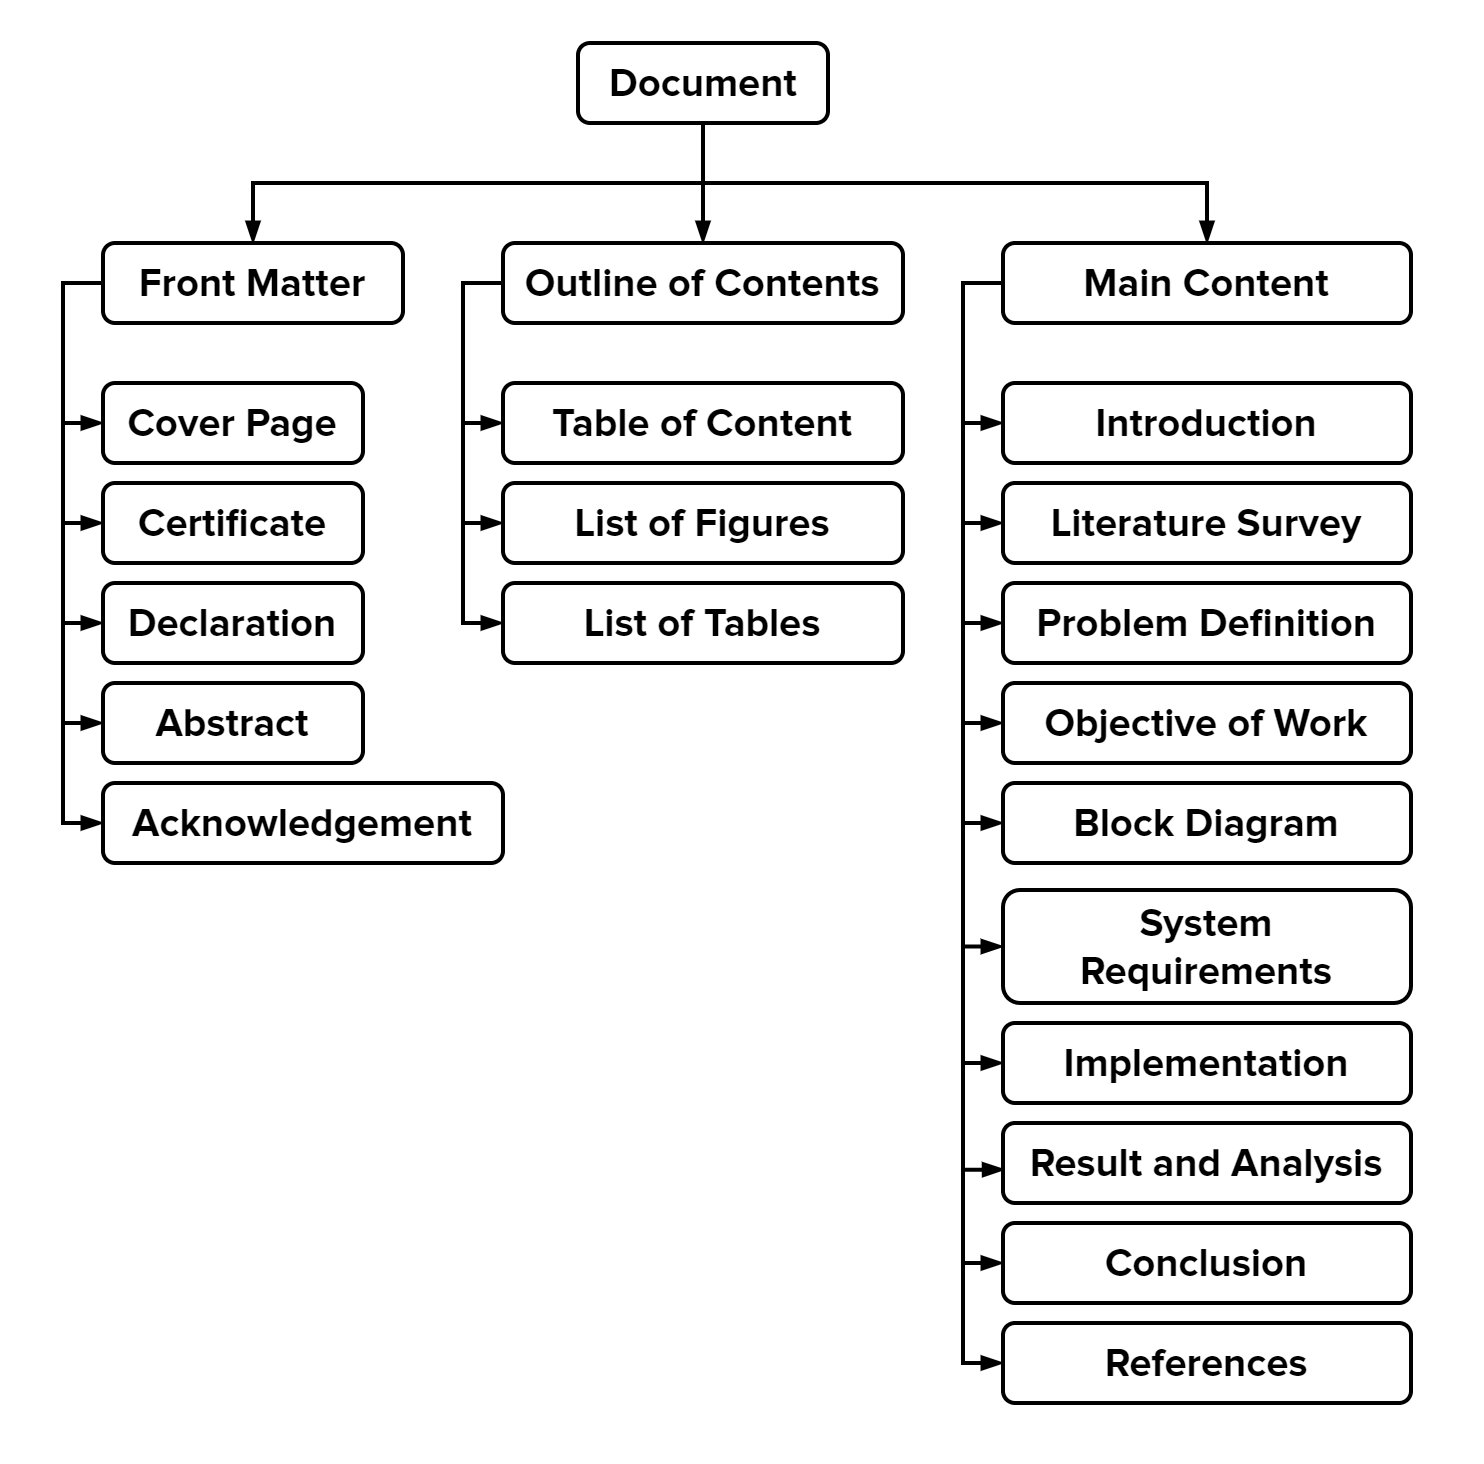
\includegraphics[width=\linewidth]{block_diagram}
	\caption{Block Diagram}
	\label{blockDiagram}
\end{figure}


% ================= Chapter 6 ================= %

% add System Requirements of your project in 
% system-requirements.tex file

\chapter{System requirements}

\section{Using Overleaf}

Overleaf provides a rich-text editor so you don't need to know any code to get started—you can just edit the text, add images, and see the typeset document automatically created for you as you type. Our tutorial provides a quick three-step introduction to the main features. \\

Overleaf is an online collaborative writing and publishing tool that makes the whole process of writing, editing and publishing scientific documents much quicker and easier. Overleaf provides the convenience of an easy-to-use LaTeX editor with real-time collaboration and the fully compiled output produced automatically in the background as you type. \\

If you're familiar with LaTeX, using Overleaf couldn't be simpler as we provide full support for direct LaTeX editing, and automatically compile your document for you on our servers (so there's nothing to install). All you need to do is create a document and choose source mode in the editor to edit the LaTeX code for your paper. \\

\noindent The key features if Overleaf are :

\begin{itemize}
    \item All you need is a web browser
    \item Always have the latest version
    \item Effortless sharing
    \item Automatic real-time preview
    \item Real-time track changes and commenting
    \item Complementary Rich Text and LaTeX modes
    \item Quickly find LaTeX errors
\end{itemize}

If you're new to LaTeX and would like to learn more about it, we recommend completing our online introduction to LATEX course, prepared by Dr John Lees-Miller and originally presented at the University of Bristol. 

\section{Using MiKTEX and Texmaker}

\noindent The recommended TEX distributions are:
\begin{itemize}
    \item TEXLive is a major TEXdistribution for Unix/Linux, Mac OS and Windows.
    \item MiKTeX is a Windows-specific distribution.
    \item MacTeX is a Mac OS-specific distribution based on TEXLive.
\end{itemize}

The Texmaker is an editor with the text window, structure window, toolbars, functions, and status bar. The white portion shows the text or writing window, and the black part shows the structure window. It contains a link to chapters, sections, tables, equations, etc. The features of Texmaker are given below:

\begin{itemize}
    \item It includes spell checking while typing.
    \item It supports a variety of encodings.
    \item It contains a 'structure view,' which gets automatically updated while typing.
    \item In Texmaker, with the use of keyboard triggers, you can define an unlimited number of snippets.
    \item It gives you the full asymptotic support.
    \item It includes the built-in PDF viewer and the 'Quick Build' command.
    \item The Texmaker includes 37O mathematical symbols, which can be inserted in just one click.
    \item The extensive Latex document is furnished with the Texmaker.
    \item It automatically detects the warnings and errors with the corresponding line number after the compilation. It also contains the detail of each error.
    \item It also allows us to work efficiently onto the documents separated in several files with the "master mode."
\end{itemize}



% ================= Chapter 7 ================= %

% add Implementation of your project in 
% implementation.tex file

\chapter{Implementation}

\section{Editing your document}

You can edit your \LaTeX \ document with any text editor. EMACS, vi, kate, gedit or even (ugh!) MicroSoft Notepad can be used. Save your document with a name that ends in .tex so that you and \LaTeX \ know that it contains \LaTeX \ source code. An absolute minimum \LaTeX \ document is:

\begin{lstlisting}
\documentclass{article}
\begin{document} 
Here is some text for \LaTeX\ to typeset. 
\end{document}
\end{lstlisting}

Note that things beginning with a are instructions to the LATEX program. Everything else is text to be typeset. 

\section{Organize}

\LaTeX \ can organize, number, and index chapters and sections of document. There are up to 7 levels of depth for defining sections depending on the document class:
\begin{lstlisting}
 -1 \part{part}
  0 \chapter{chapter}
  1 \section{section}
  2 \subsection{subsection}
  3 \subsubsection{subsubsection}
  4 \paragraph{paragraph}
  5 \subparagraph{subparagraph}
\end{lstlisting}

Usually, \verb|\section| is the top-level document command in most documents. However, in reports or books, and similar long documents, this would be \verb|\chapter| or \verb|\part|. \\

In our template we have used report document so \verb|\chapter| is the top-level document command.

\section{Sectioning}

You can generate section, subsection, subsubsection headings using \verb|\section| etc. The sections are numbered automatically.

\subsection{Avoiding numbering}

If you want a section without its number, put a star on the end of the command, like this: Un numbered subsubsection Generated with the \verb|\subsubsection*{}| command.

\subsection{Unnumbered sections in the table of contents}

To add an unnumbered section to the table of contents, use the \verb|\addcontentsline| command like this:
\begin{lstlisting}
\addcontentsline{toc}{section}{Title of the section}
\end{lstlisting}

\section{Chapters}

The \LaTeX \ default starts each chapter on a fresh page, an odd-numbered page if the document is two-sided. It produces a chapter number such as ‘Chapter 1’ in large boldface type (the size is \verb|\huge|). It then puts title on a fresh line, in boldface type that is still larger (size \verb|\Huge|). It also increments the chapter counter, adds an entry to the table of contents, and sets the running header information.

This produces a chapter.

\begin{lstlisting}
\chapter{Loomings}
Call me Ishmael.
    Some years ago--
\end{lstlisting}

In our template we have seperated chapter for each topic. The list goes as

\begin{lstlisting}
\chapter{Introduction}
\chapter{Literature Review}
\chapter{Problem Definition}
\chapter{Objective of Work}
\chapter{Models/Block diagram}
\chapter{System requirements}
\chapter{Implementation}
\chapter{Results and Analysis}
\chapter{Conslusion anf Future Scope}
\end{lstlisting}

\section{Including figures}

Figures are inserted using the \verb|\includegraphics| command. For this to work, you need to have used \verb|\usepackage{graphicx}| near the start of the document. You can use \verb|\includegraphics| anywhere you like. \\

\begin{figure}[htb]
    \noindent\hrulefill
	\centering
	\caption{This picture is in a float, which means that \LaTeX \ will put it in a suitable position, somewhere close to where you put it in your LATEX source.}
	
\includegraphics[width=0.3\linewidth]{butterfly}
	\label{butterflyCenter}\par
    \hrulefill
\end{figure}

The below figure has to appear exactly where I put it, between “. . . you like.” and “The above figure. . . ”. This is not smart for anything except the smallest graphics, because it can lead to large spaces at the foot of a page. More usually, we put figures into a float, like figure \ref{butterflyCenter}. \\

The source code for a floating figure looks like this:

\begin{lstlisting}
\begin{figure}[h!] 
Figure content goes here 
\caption{\label{myfiglabel} Your caption goes here} 
\end{figure}
\end{lstlisting}

Note that LATEX provides a numbered caption. Make sure you put your \verb|\label{}| inside the caption or the cross-referencing may not work properly. \\

The optional \verb|[htbp]| argument gives you a little control over where the figure goes: you can put any combination of here \verb|[h]|, top (of a page) \verb|[t]| , bottom of a page \verb|[b]|, (whole) page (containing only figures) \verb|[p]| and LATEX will do its best give you the best of the options you permitted. Note that you need to be relaxed about figures not appearing exactly “here”. For this reason, always refer to a figure by its number, never as “the figure below” or “the figure above”. (This is good practice for real life: when you write a paper for a scientific journal, the journal staff always take control over figure placement and you never know where they are going to put the figures.) New LATEX users often try to be too restrictive about figure placement; this often results in LATEX deciding that there is no good answer and putting all of your figures right at the end of the document. \\

The caption is usually positioned below the figure. With a bit more work you can position the caption at the side of the figure; if your figure is square-ish this saves you some space. Figure \ref{butterflyLeft} shows how this is done. \\

\noindent\hrulefill
\begin{figure}[htbp]
  \begin{minipage}[c]{0.3\linewidth}
    
\includegraphics[width=\linewidth]{butterfly}
  \end{minipage}\hfill
  \begin{minipage}[c]{0.7\linewidth}
    \caption{For this figure, the caption is placed inside a minipage; this is a small block of text which is typeset as a unit and then treated as a single item, as if it were a picture, or a very large character.} 
    \label{butterflyLeft}
  \end{minipage}
\end{figure}
\par
\noindent\hrulefill
  
LATEX can not include all types of graphics, so you need to make your pictures in the correct format, or convert them to it.

\begin{itemize}
    \item If you use latex and dvips then all of your figures must be encapsulated PostScript.
    \item If you use pdflatex then your figures may be any of
    \begin{itemize}
        \item Portable Document Format (PDF)
        \item JPEG image
        \item PNG image
    \end{itemize}
\end{itemize}

If you miss off the filetype extension, then LATEX will look for a file with a suitable extension. So if you do 

\begin{lstlisting}
\includegraphics[width=4cm]{lara_croft}
\end{lstlisting}

then latex will look for a file called \verb|lara_croft.eps|, but pdflatex will look for files called \verb|lara_croft.pdf|, \verb|lara_croft.jpg| and \verb|lara_croft.png| (in I don’t know what order). 

\section{Tables}

The \verb|tabular| environment is the default LATEX method to create tables. You must specify a parameter to this environment; here we use \verb|{c c c}| which tells LaTeX that there are three columns and the text inside each one of them must be centred.

\subsection{Creating a simple table in LATEX}

The tabular environment provides additional flexibility; for example, you can put separator lines in between each column:

\begin{lstlisting}
\begin{tabular}{ |c|c|c| } 
    \hline
    cell1 & cell2 & cell3 \\ 
    cell4 & cell5 & cell6 \\ 
    cell7 & cell8 & cell9 \\ 
    \hline
\end{tabular}
\end{lstlisting}

This produces :

\begin{tabular}{ |c|c|c| } 
    \hline
    cell1 & cell2 & cell3 \\ 
    cell4 & cell5 & cell6 \\ 
    cell7 & cell8 & cell9 \\ 
    \hline
\end{tabular}

\section{Page Layout}

Fitting a LATEX document to a strict page layout can be a bit fraught. I set this document up so that it matched the requirements of the projects course organiser:

\begin{itemize}
    \item 12 point font
    \item 2.5 cm margins
    \item 1.0 line spacing
    \item A space (size unspecified) between paragraphs
\end{itemize}

But the exact size and position on the paper may be messed up a bit in the printing process. The important thing is to ensure that page scaling and auto-centre and rotate are turned OFF when you print the page. In the evince document viewer, the print dialog has a “Page Handling” tab; select “Page Scaling=None” and uncheck the “Auto-Rotate and Centre” box. The print dialog in Adobe reader has a page handling section with similar controls. 

\begin{lstlisting}
\textheight=23cm 
\topmargin=0.5cm 
\oddsidemargin=0.5cm 
\textwidth=15.0cm 
\end{lstlisting}

\section{Fonts and sizes}

Try to avoid controlling font size by hand. LATEX’s default style is pre-set to use sensible font sizes for most things. If you insist, LATEX comes with several pre-defined sizes: {\tiny tiny}, {\scriptsize scriptsize}, {\footnotesize footnotesize}, {\small small}, {\normalsize normalsize}, {\large large}, {\large large}, {\LARGE LARGE}, {\huge huge}, and {\Huge Huge}.

\section{Page Border}

Page border for a certain page can be added using following code :

\noindent\verb|\begin{tikzpicture}[overlay,remember picture]|\\
\verb|    \draw [line width=3pt]|\\
\verb|        ($ (current page.north west) + (1.3cm,-1.3cm) $)|\\
\verb|            rectangle|\\
\verb|        ($ (current page.south east) + (-1.3cm,1.3cm) $);|\\
\verb|    \draw [line width=1pt]|\\
\verb|        ($ (current page.north west) + (1.45cm,-1.45cm) $)|\\
\verb|            rectangle|\\
\verb|        ($ (current page.south east) + (-1.45cm,1.45cm) $); |\\
\verb|\end{tikzpicture}|\\

In our template, we have added page border in cover page, certificate and declaration page.

\section{User defined variables}

\begin{lstlisting}
\def<cs><arg syntax>{<definition>}
\end{lstlisting}

This defines \verb|<cs>| without checking if it already exists. The ⟨definition⟩ part is the same as that for \verb| \newcommand|, but with \verb|\def| you don't just specify the number of arguments. Instead you declare the argument syntax in \verb|<arg syntax>| where each parameter is identified by \verb|#<n>| (where\verb|<n>| is a number from 1 to 9).

The simplest form is when you define a command that has no arguments. For example:

\begin{lstlisting}
\def\test{This is a test.}% definition
\test
\end{lstlisting}

produces:

\def\test{This is a test.}% definition
\test

\verb|\def| can be preceded by \verb|\global| (the redefinition isn't confined to the current group, also controlled by \verb|\globaldefs|), \verb|\long| (the command admits long arguments), \verb|\outer| (the command is not tolerated in parts of the code which are read at high speed).

\verb|\gdef| works as \verb|\def| except that the definition is automatically set as \verb|\global|, or in other words, visible from the outside of the current group. In our template we have created \verb|\gdef| definitions such as

\begin{lstlisting}
\gdef \title {Technical Project Report Template using Latex} 
\gdef \dept {Information Technology} 
\gdef \degree {Bachelor of Engineering} 
\gdef \branch {Information Technology} 
\gdef \college {Bharati Vidyapeeth College of Engineering} 
\gdef \collegeplace {Navi Mumbai} 
\gdef \studentA {Bhoir Ankit Bharat} 
\gdef \studentAroll {4407} 
\gdef \studentB {Chouhan Aman Ravi} 
\gdef \studentBroll {4414} 
\gdef \studentC {Badge Aman Ramesh} 
\gdef \studentCroll {4404} 
\gdef \studentD {Ankolekar Vaibhav Pandurang} 
\gdef \studentDroll {4401} 
\gdef \guide {Prof. Hanamant B. Sale}
\gdef \guidedes {Subject Co-ordinator}
\gdef \hod {Dr. Shankar M. Patil} 
\gdef \hoddes {Head of Department} 
\end{lstlisting}

% ================= Chapter 8 ================= %

% add Results and Analysis of your project in 
% results-and-analysis.tex file

\chapter{Results and Analysis}

\begin{figure}[h!]
	\centering
	\frame{
	    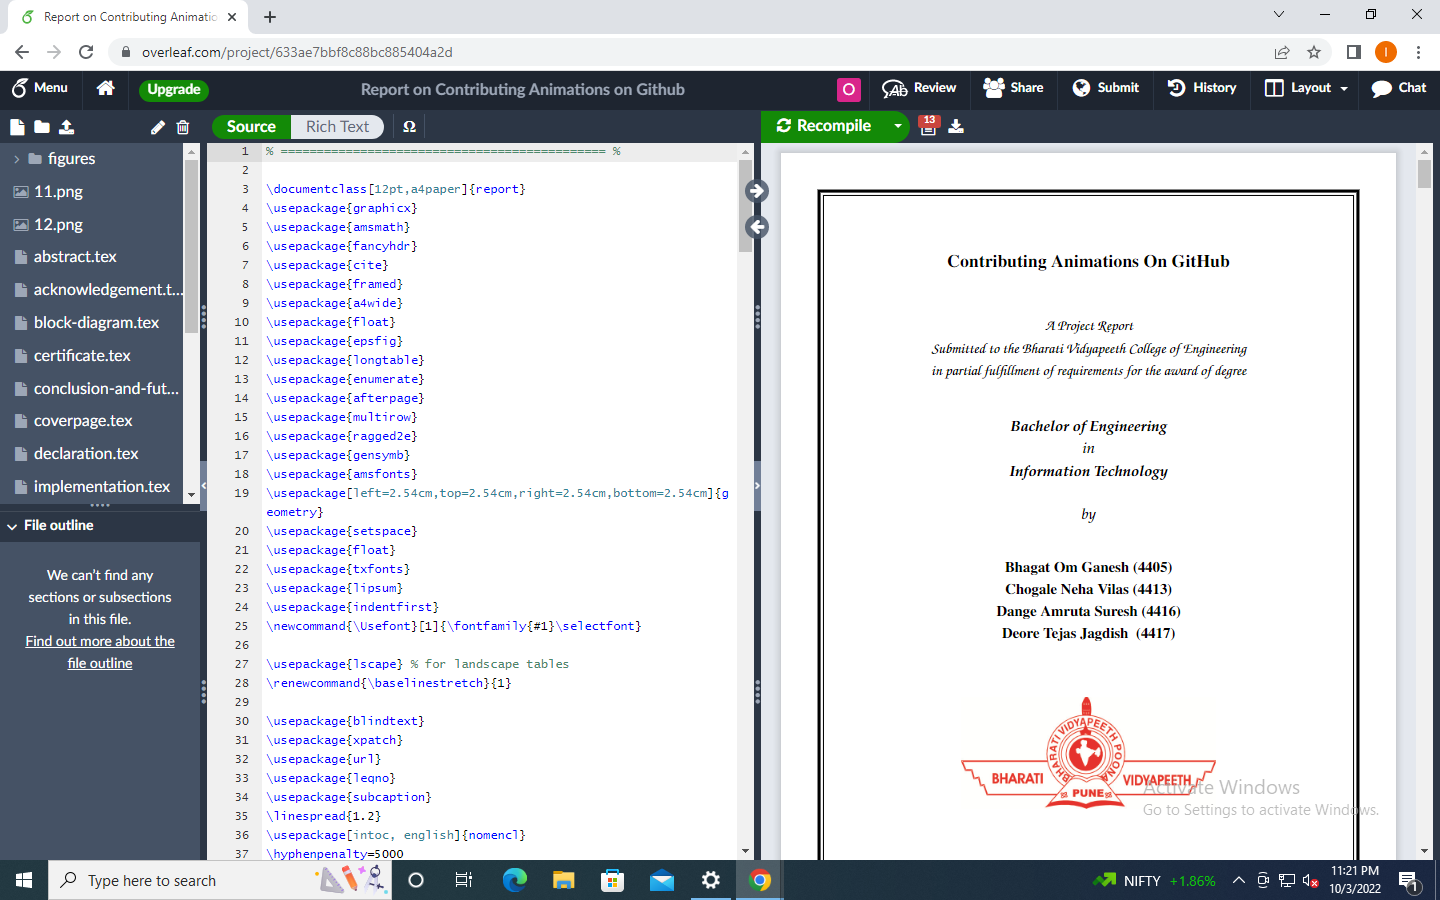
\includegraphics[width=1\linewidth]{result1}
	}
	\caption{Result of cover-page with border}
	\label{resul1}
\end{figure}

\begin{figure}[h!]
	\centering
	\frame{
	    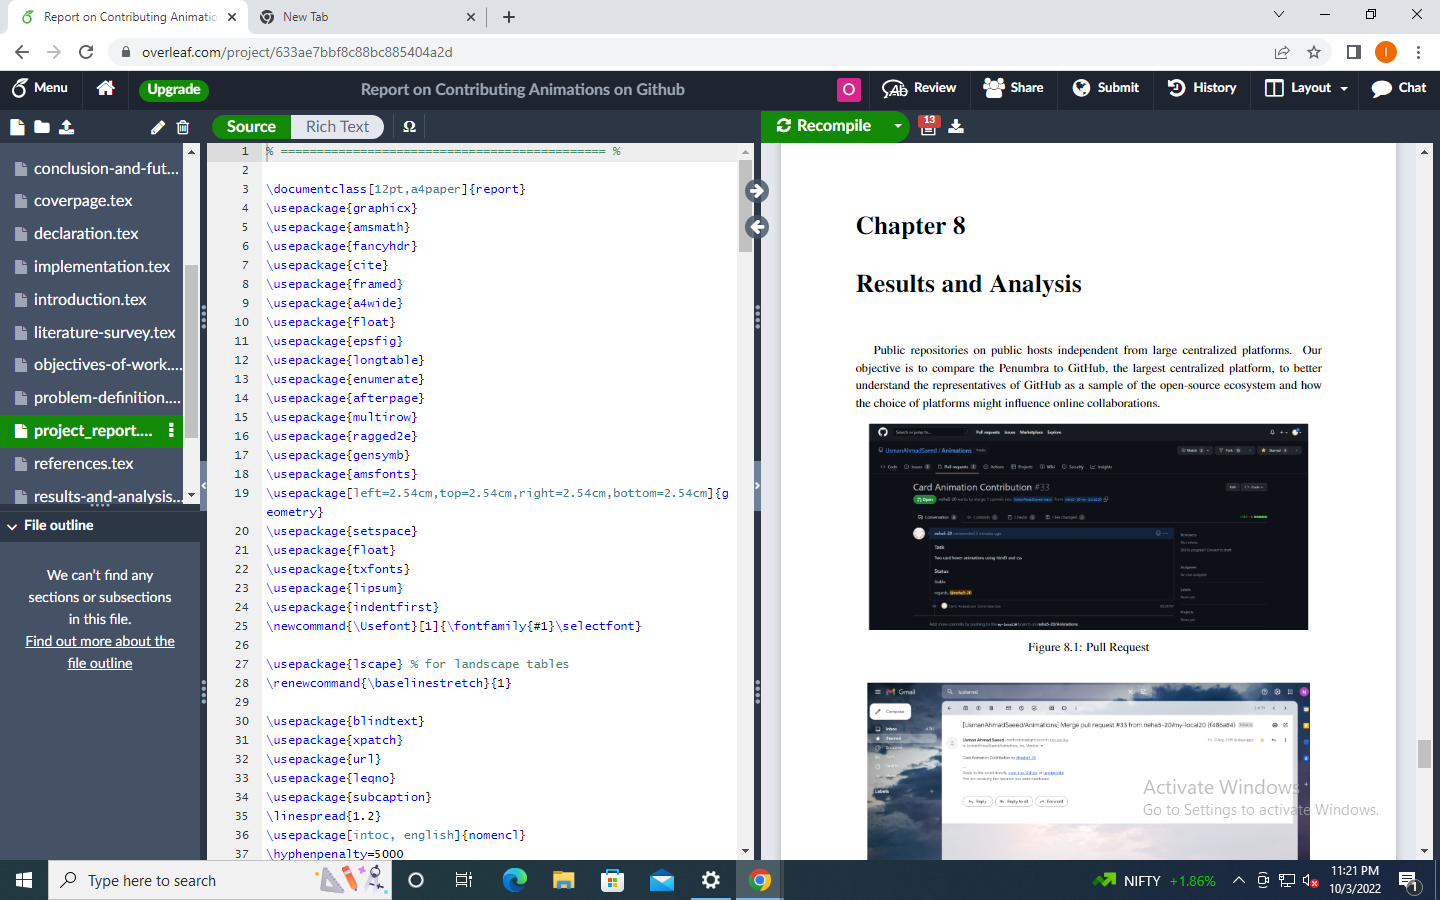
\includegraphics[width=1\linewidth]{result2}
	}
	\caption{Result of images added in template}
	\label{result2}
\end{figure}

% ================= Chapter 9 ================= %

% add Conclusion and Future Scope of your project 
% in conclusion-and-future-scope.tex file

\chapter{Conclusion and Future Scope}

\section{Conclusion}

Thus our project “\title" concentrates on the documentation of project reports which includes project title page, certificate etc. The standard formatting constraints for these documents are defined in packages developed under this project, which will thus help the user to complete his/her work in stipulated time and making it less tedious. This template is used by other project groups of Information Technology department of Bharati Vidyapeeth College of Engineering. This template can also be used by other College or Universities by doing some changes in names and college logo.

\section{Future Scope}

In order to make use of class files developed in the project, the basic requirement is that the user must have the sound knowledge of \LaTeX. So to make it more handy, user interface can be developed which will take only the required values as input viz; the content of notice and the packages in the back-end will take care of formatting without the user having to know \LaTeX \ commands.

% ================= References ================= %

% add References of your project in 
% references.tex file


% This template uses IEEE bibliography style 

\begin{thebibliography}{99}
	
% 	\bibitem{india} HU, Yun Chao, et al., \emph{Mobile edge computing?A key technology towards 5G}, ETSI white paper, 2015, vol. 11, no 11, p. 1-16.
	
% 	\bibitem{rpi}
% 	@online Raspberry pi, \url{https://www.raspberrypi.org/} Online; accessed 10-June-2019
	
% 	\bibitem{japan} HU, Yun Chao, et al., \emph{Mobile edge computing?A key technology towards 5G}, ETSI white paper, 2015, vol. 11, no 11, p. 1-16.
	
	\bibitem{overleaf} \url{https://www.overleaf.com/learn}
	
	\bibitem{overleaf} \url{https://miktex.org/docs}
	
	\bibitem{southampton} \url{https://www.southampton.ac.uk/~fangohr/computing/latex/latex_for_report_writing_HF.pdf}
	
	\bibitem{ctan}
	\url{http://tug.ctan.org/tex-archive/macros/latex/contrib/famt/ProjectReport/Report.pdf}
	
	\bibitem{citeseerx}
	\url{https://citeseerx.ist.psu.edu/viewdoc/download?doi=10.1.1.365.502&rep=rep1&type=pdf}
	
	\bibitem{geos}
	\url{https://www.geos.ed.ac.uk/~hcp/latex_examples/gp_project_in_latex.pdf}
	
	\bibitem{srmcollege}
	\url{https://www.srmcollege.in/wp-content/uploads/2020/02/Report-wrtining-using-Latex.pdf}
	
	\bibitem{phys}
	\url{https://www.phys.ufl.edu/courses/phy4803L/sample-paper.pdf}
	
\end{thebibliography}

\end{document}